\section{Modularisierung}
Ziel ist es eine schwache \textbf{Kopplung} und starke Kohäsion zu bekommen.

Kopplung: Sie sollten die Kopplung der Komponenten gering halten. Die einzelnen Klassen, Module etc. sollten so wenig voneinander wissen wie möglich. Das Ziel ist die Abhängigkeiten zwischen den einzelnen Modulen möglichst gering zu halten. In der OOP finden sich hierzu viele hilfreiche Entwurfsmuster und auch das Information Hiding der Details von Modulen sollten Sie verwenden. Wählen sie dazu immer die kleinstmöglichste Sichtbarkeit eines Details

\begin{center}
	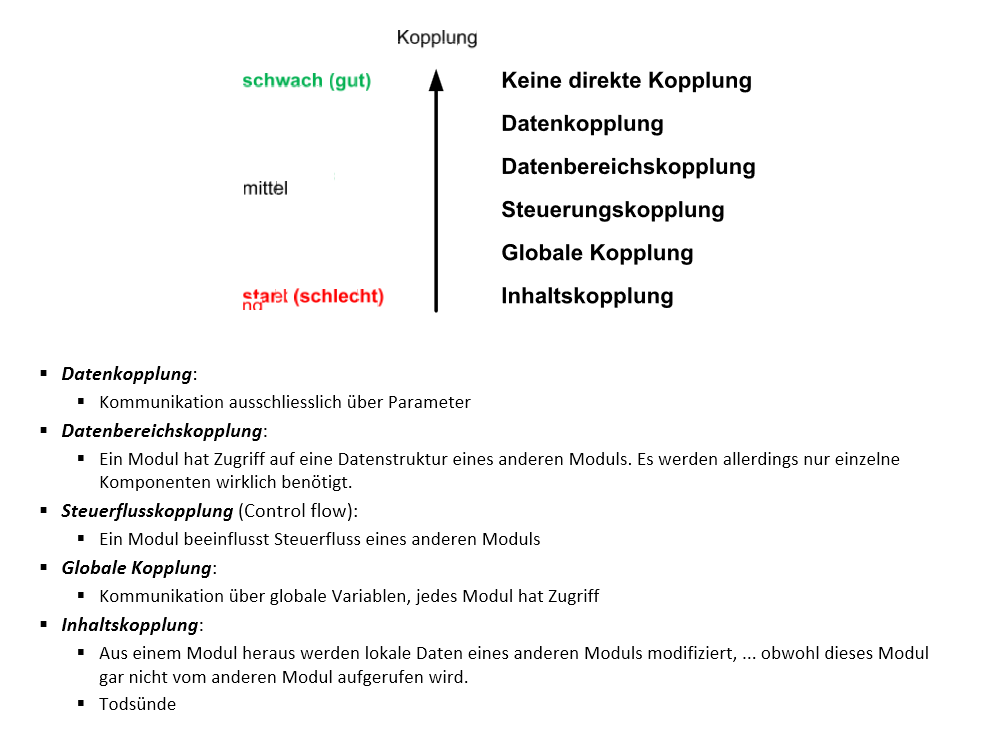
\includegraphics[width=\columnwidth]{Images/kopplung}
\end{center}

Kohäsion: Wenn Sie eine Klasse implementieren, sollte darauf geachtet werden, dass diese Klasse nicht mehrere Verantwortlichkeiten in sich trägt. Kohäsion ist ein Mass für den logischen Zusammenhang der Daten und Methoden der Klasse. Sie sollten keine Verantwortlichkeiten und Aufgaben innerhalb einer Klasse vermischen.
\begin{center}
	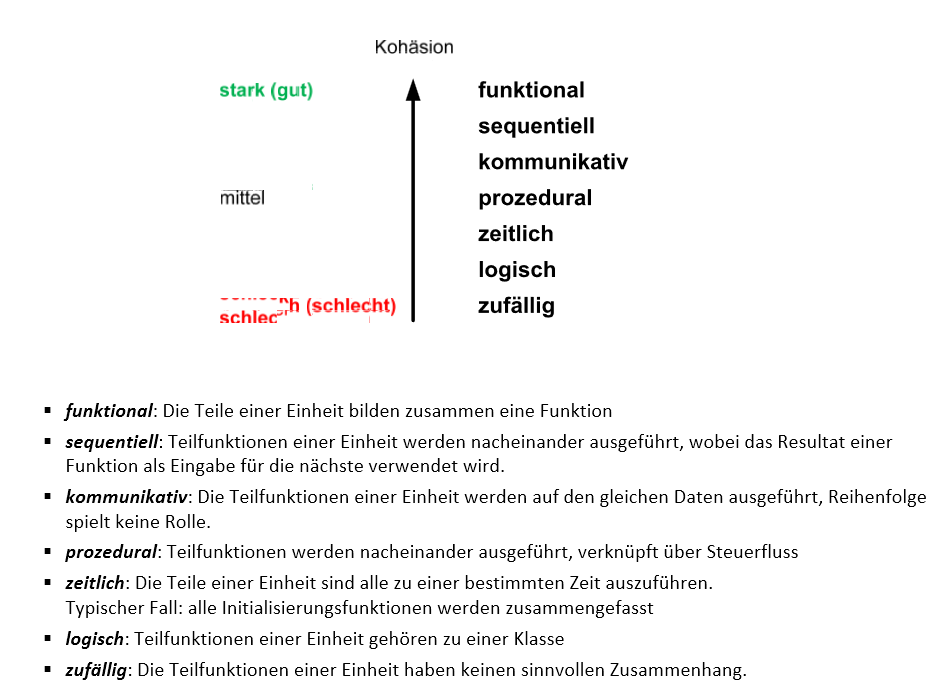
\includegraphics[width=\columnwidth]{Images/kohäsion}
\end{center}

